%&-job-name=newfilenameialwayswanted
\documentclass[
a4paper, % Stock and paper size.
12pt, % Type size.
article,
% oneside, 
onecolumn, % Only one column of text on a page.
% openright, % Each chapter will start on a recto page.
% openleft, % Each chapter will start on a verso page.
openany, % A chapter may start on either a recto or verso page.
]{memoir}
\synctex=1
\maxtocdepth{subsection}
\setsecnumdepth{subsection}
\counterwithout{section}{chapter}
%%% PACKAGES 
%%%------------------------------------------------------------------------------
\usepackage[utf8]{inputenc} % If utf8 encoding
% \usepackage[lantin1]{inputenc} % If not utf8 encoding, then this is probably the way to go
\usepackage[T1]{fontenc}    %
\usepackage[english,russian]{babel} % English please


%%% Figures and colors
\usepackage[usenames,dvipsnames,svgnames,table,rgb]{xcolor}
\usepackage{tikz} % Figures. Following colors are predefined: red, green, blue, cyan, magenta, yellow, black, gray, darkgray, lightgray, brown, lime, olive, orange, pink, purple, teal, violet and white.

% Defining a new coordinate system for the page:
%
% --------------------------
% |(-1,1)    (0,1)    (1,1)|
% |                        |
% |(-1,0)    (0,0)    (1,0)|
% |                        |
% |(-1,-1)   (0,-1)  (1,-1)|
% --------------------------
\makeatletter
\def\parsecomma#1,#2\endparsecomma{\def\page@x{#1}\def\page@y{#2}}
\tikzdeclarecoordinatesystem{page}{
    \parsecomma#1\endparsecomma
    \pgfpointanchor{current page}{north east}
    % Save the upper right corner
    \pgf@xc=\pgf@x%
    \pgf@yc=\pgf@y%
    % save the lower left corner
    \pgfpointanchor{current page}{south west}
    \pgf@xb=\pgf@x%
    \pgf@yb=\pgf@y%
    % Transform to the correct placement
    \pgfmathparse{(\pgf@xc-\pgf@xb)/2.*\page@x+(\pgf@xc+\pgf@xb)/2.}
    \expandafter\pgf@x\expandafter=\pgfmathresult pt
    \pgfmathparse{(\pgf@yc-\pgf@yb)/2.*\page@y+(\pgf@yc+\pgf@yb)/2.}
    \expandafter\pgf@y\expandafter=\pgfmathresult pt
}
\makeatother

\usepackage{graphicx}  % Include figures
\usepackage{wrapfig}
\graphicspath{{img/}{../img/}} 


%%% INTERNAL HYPERLINKS
%%%-------------------------------------------------------------------------------

\usepackage{hyperref}   % Internal hyperlinks
\newcommand{\linkcolor}{blue}
\newcommand{\citecolor}{blue}
\newcommand{\filecolor}{magenta}
\newcommand{\urlcolor}{NavyBlue}
\hypersetup{				% Гиперссылки
    pdfborder={0 0 0},      % No borders around internal hyperlinks
	unicode=true,           % русские буквы в раздела PDF\\
	pdfstartview=FitH,
	colorlinks=true,  % false: ссылки в рамках; true: цветные ссылки
	linkcolor=\linkcolor,         % внутренние ссылки
	citecolor=\citecolor,        % на библиографию
	filecolor=\filecolor,      % на файлы
	urlcolor=\urlcolor,      % на URL
    linkbordercolor=\linkcolor,  % hyperlink border will be red 
    pdftitle={Yoga Veera Kit},
    pdfpagemode=FullScreen,
    pdfauthor={I am the Author} % author
}

\let\oldhref\href
\renewcommand{\href}[2]{\oldhref{#1}{\underline{#2}}}

   
\graphicspath{{img/}{../img/}{../../FreqImg/}}


%%% PAGE LAYOUT 
%%%------------------------------------------------------------------------------

\setlrmarginsandblock{0.15\paperwidth}{*}{1} % Left and right margin
\setulmarginsandblock{0.10\paperwidth}{*}{1}  % Upper and lower margin
\checkandfixthelayout
%%% indenting
\setlength{\parindent}{0em}
\setlength{\parskip}{0.5em}
\begin{document}
\begin{center}
    \Huge \textbf{AirTable Spam Filtering}
\end{center}
\tableofcontents

\tikz[remember picture,overlay] \node[opacity=0.9,inner sep=0pt] at (page cs:0.8,0.8){
\includegraphics[width=0.1\paperwidth]{IshaLogo}};




\section{Фильтрация спама от AitTable}
\subsection{Gmail}
\begin{enumerate}
    \item Откройте любое \emph{нежелательное} письмо.
	    \begin{center} 
	        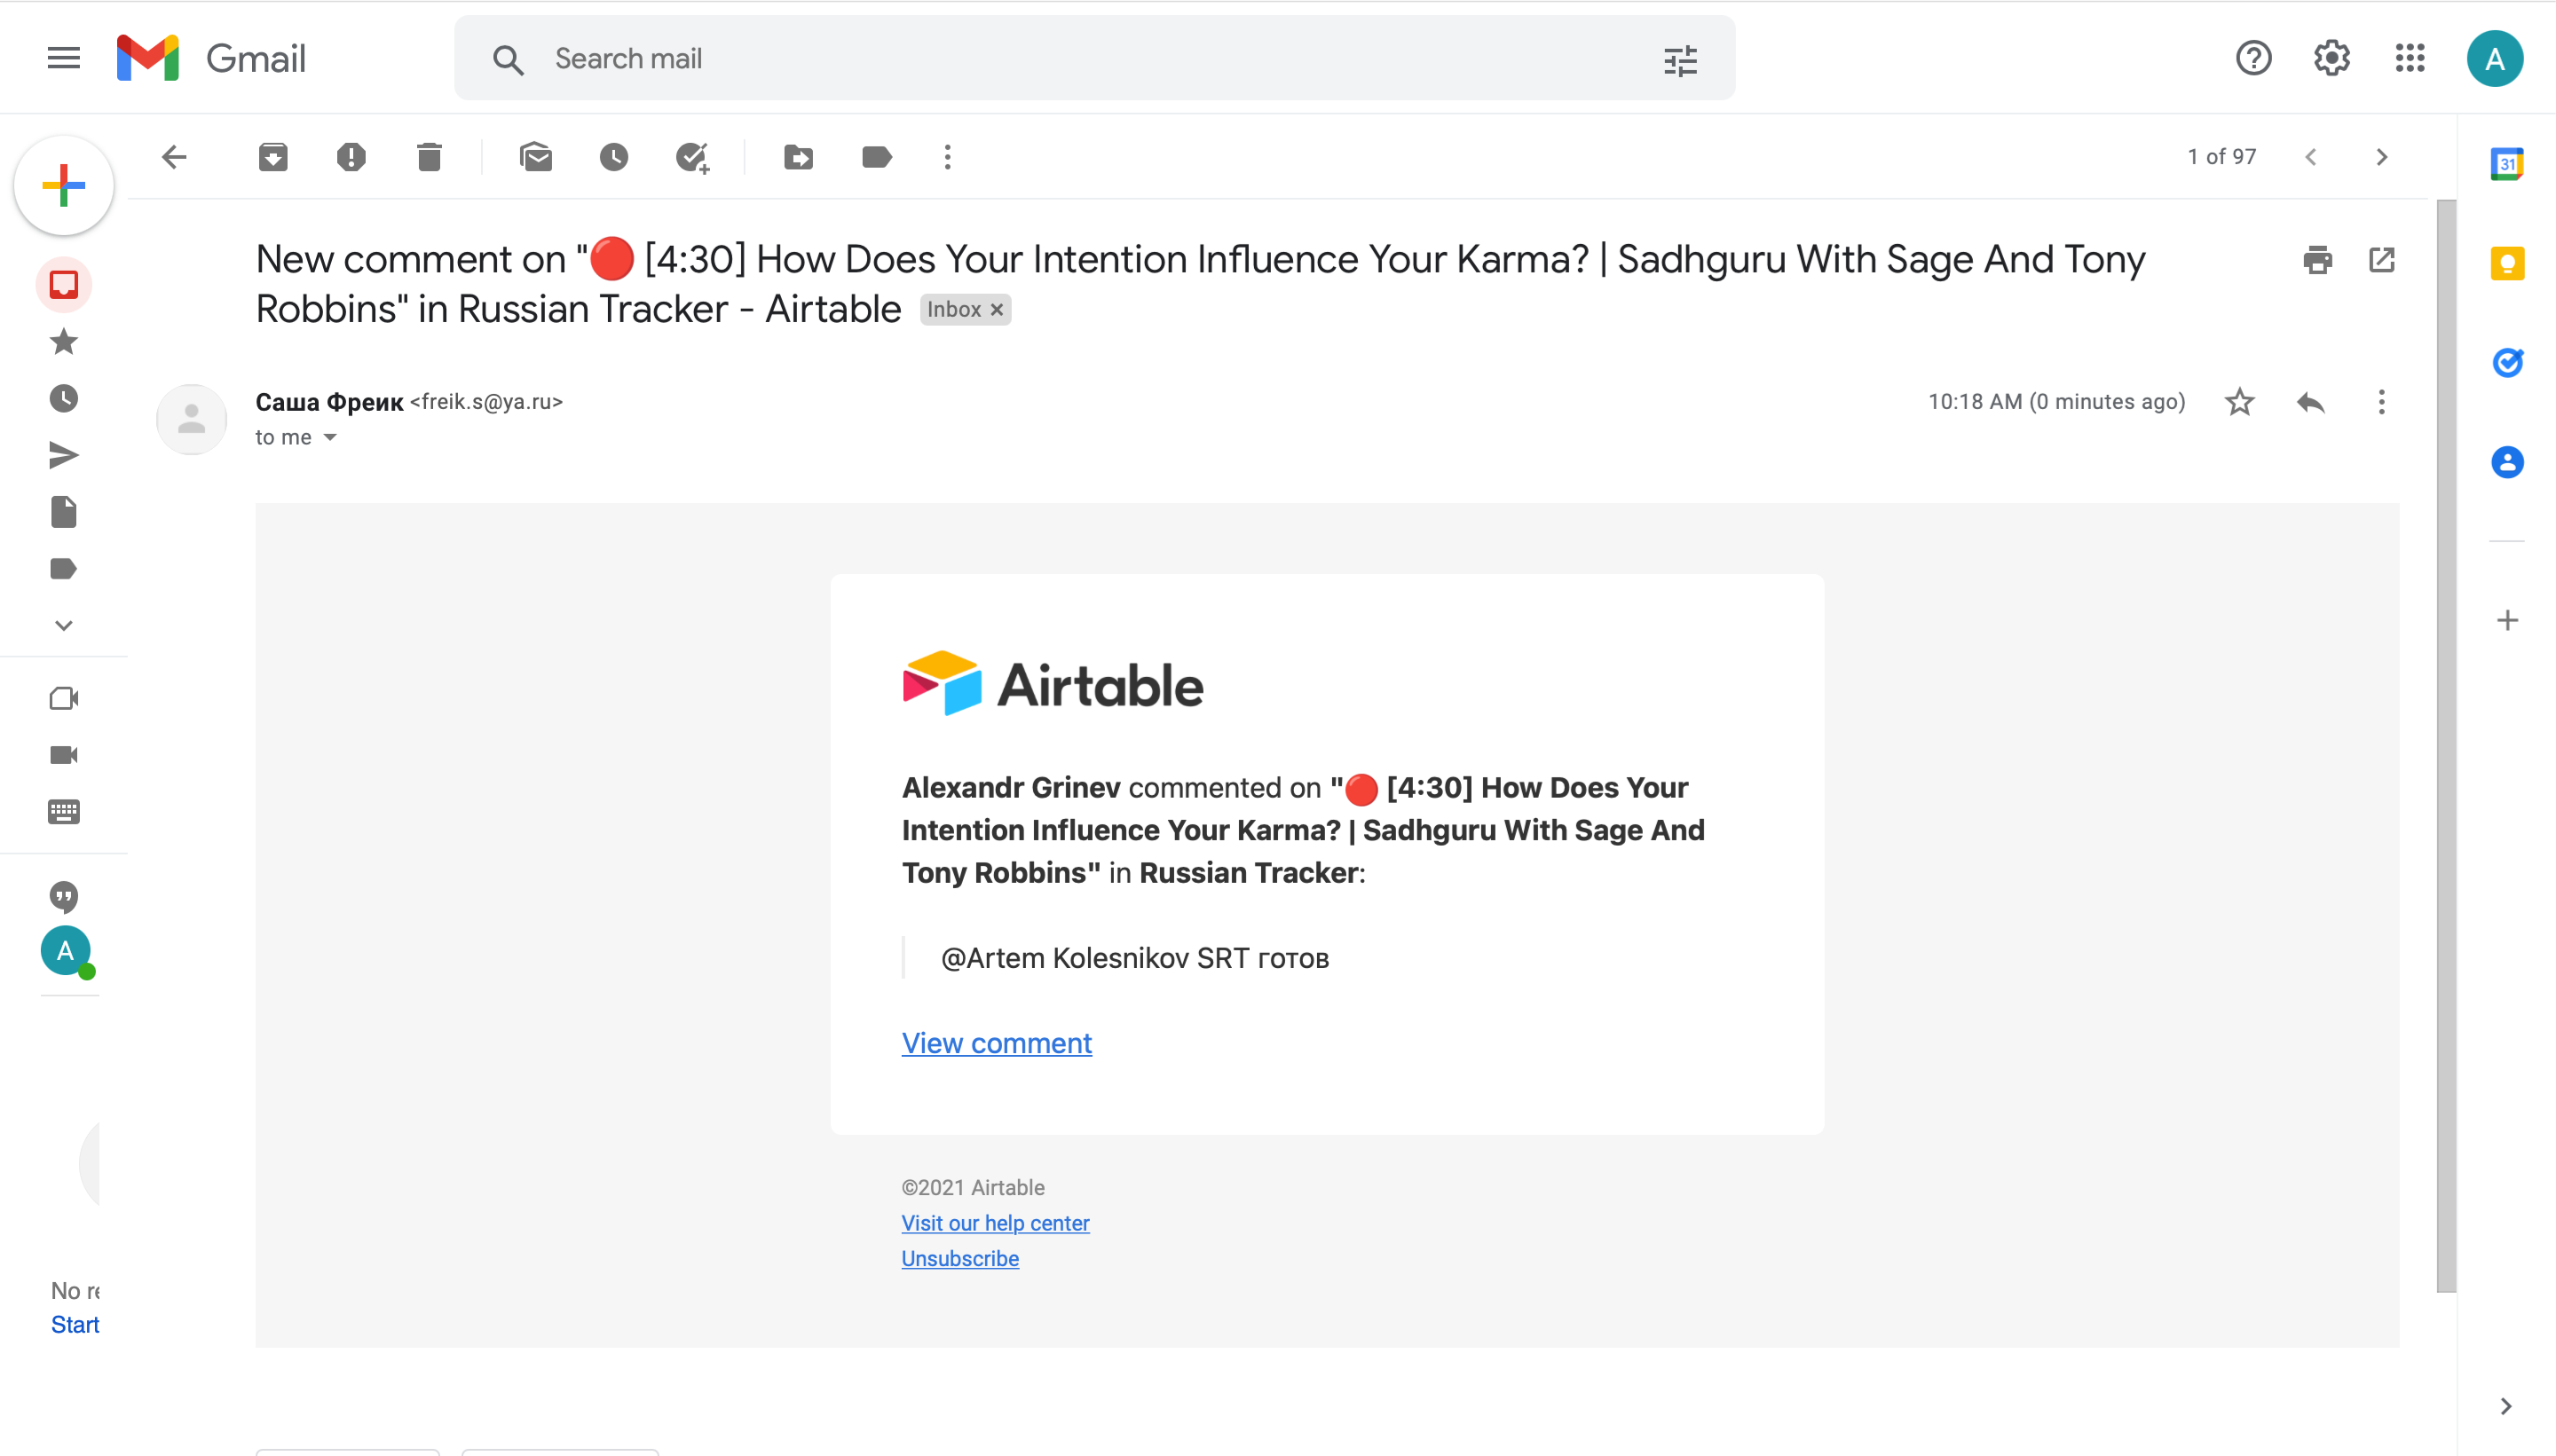
\includegraphics[width=0.9\textwidth]{AirTableSpam/gmail0} 
	    \end{center}
    \item Нажмите значек \textbf{"More"} и выберите 
                \textbf{"Filter messages like these"}.
	    \begin{center} 
	        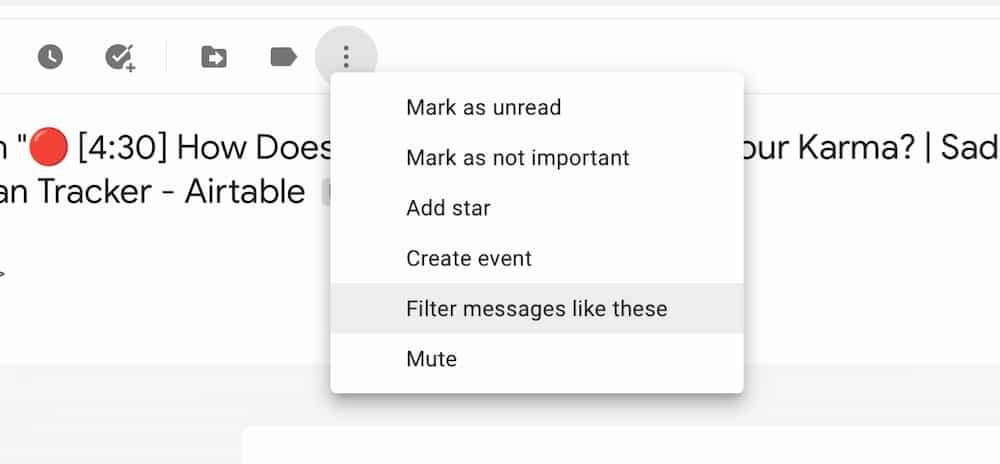
\includegraphics[width=0.5\textwidth]{AirTableSpam/gmail1} 
	    \end{center}
    \item В открывшемся окне настройте параметры, как показано ниже. 
        Далее нажмите \textbf{"Create filter"}.
        \begin{itemize}
            \item From: \textbf{"noreply@airtable.com"}
            \item Subject: \textbf{"New comment on "}
        \end{itemize}

	    \begin{center} 
	        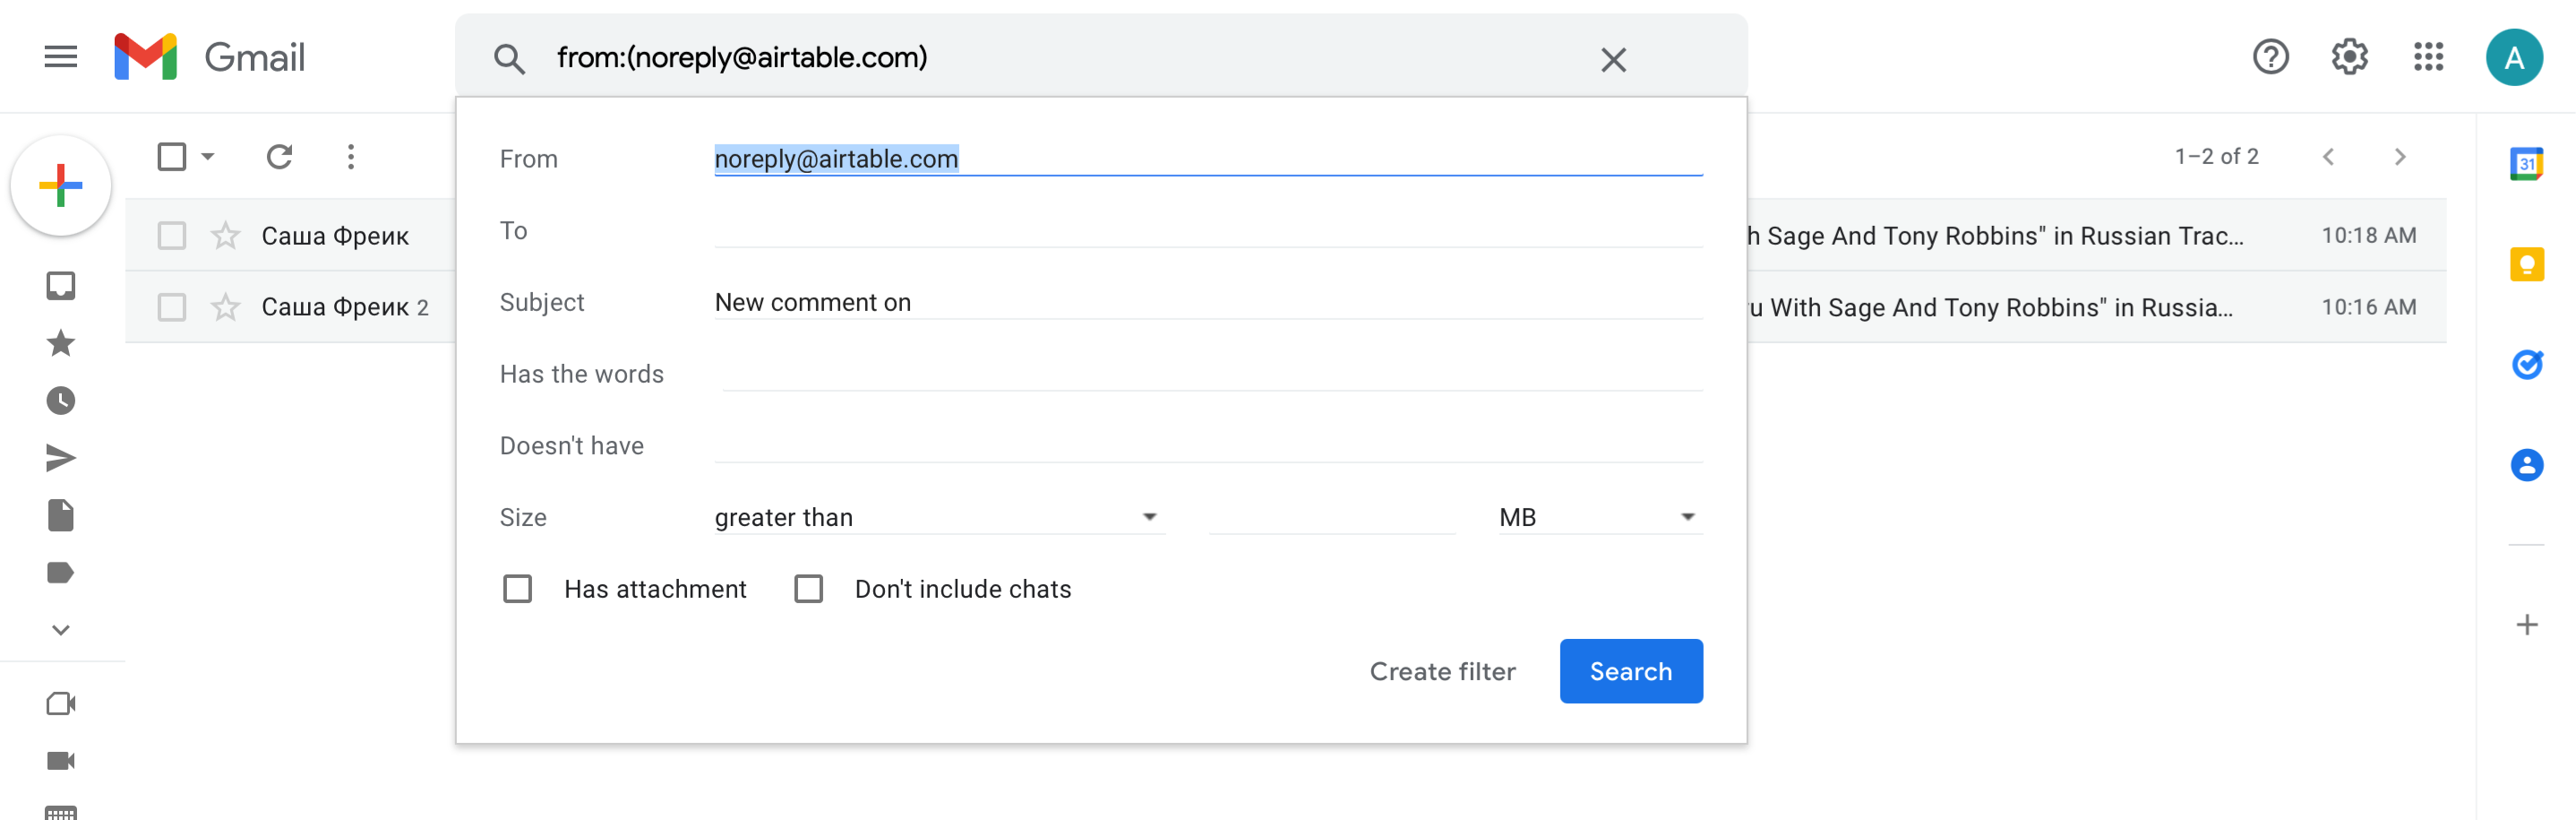
\includegraphics[width=0.9\textwidth]{AirTableSpam/gmail2} 
	    \end{center}
    \item Отметьте параметры \textbf{"Skip the Inbox (Archive it)"} и
        \textbf{"Mark as read"}, как показано ниже. 
        \begin{itemize}
            \item Далее все письма от \textbf{"noreply@airtable.com"}, 
                предмет которых которых содержит "New comment on "
                будут автоматически помечаться прочитанными и 
                перемещаться в папку \textbf{"Archive"}.
            \item Если отметить калочкой \textbf{"Also apply filter to ..."},
                то фильтр применится и к \emph{нежелательным} письмам, 
                которые уже пришли.
        \end{itemize}

	    \begin{center} 
	        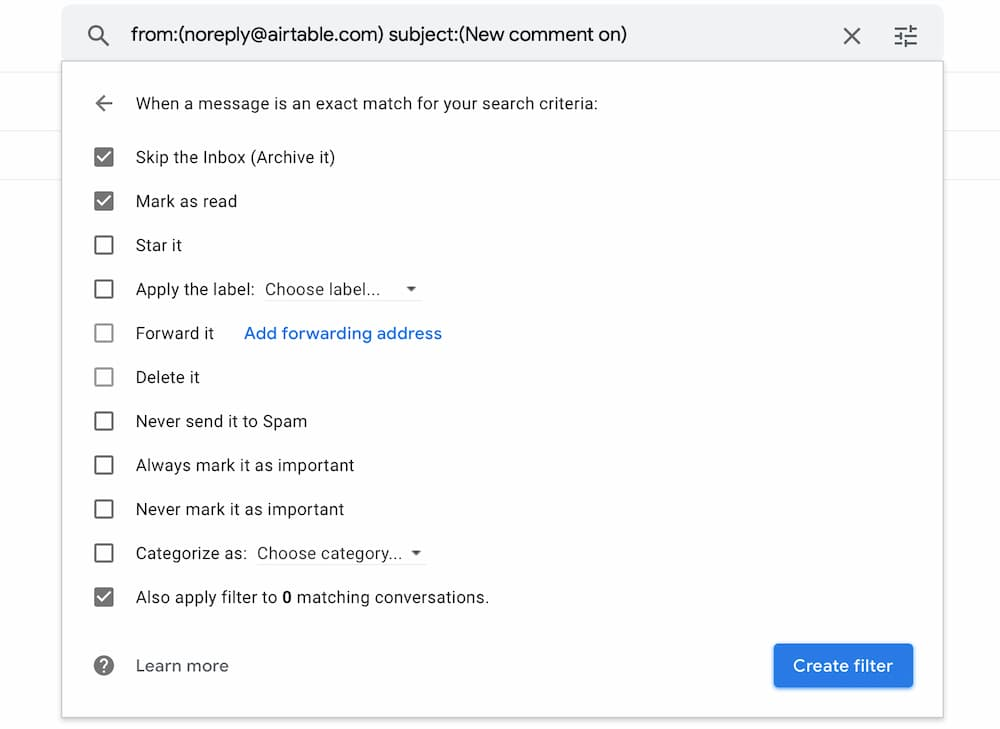
\includegraphics[width=0.7\textwidth]{AirTableSpam/gmail3} 
	    \end{center}
\end{enumerate}


\newpage
\subsection{Yandex mail}
\begin{enumerate}
    \item Откройте любое \emph{нежелательное} письмо.
	    \begin{center} 
	        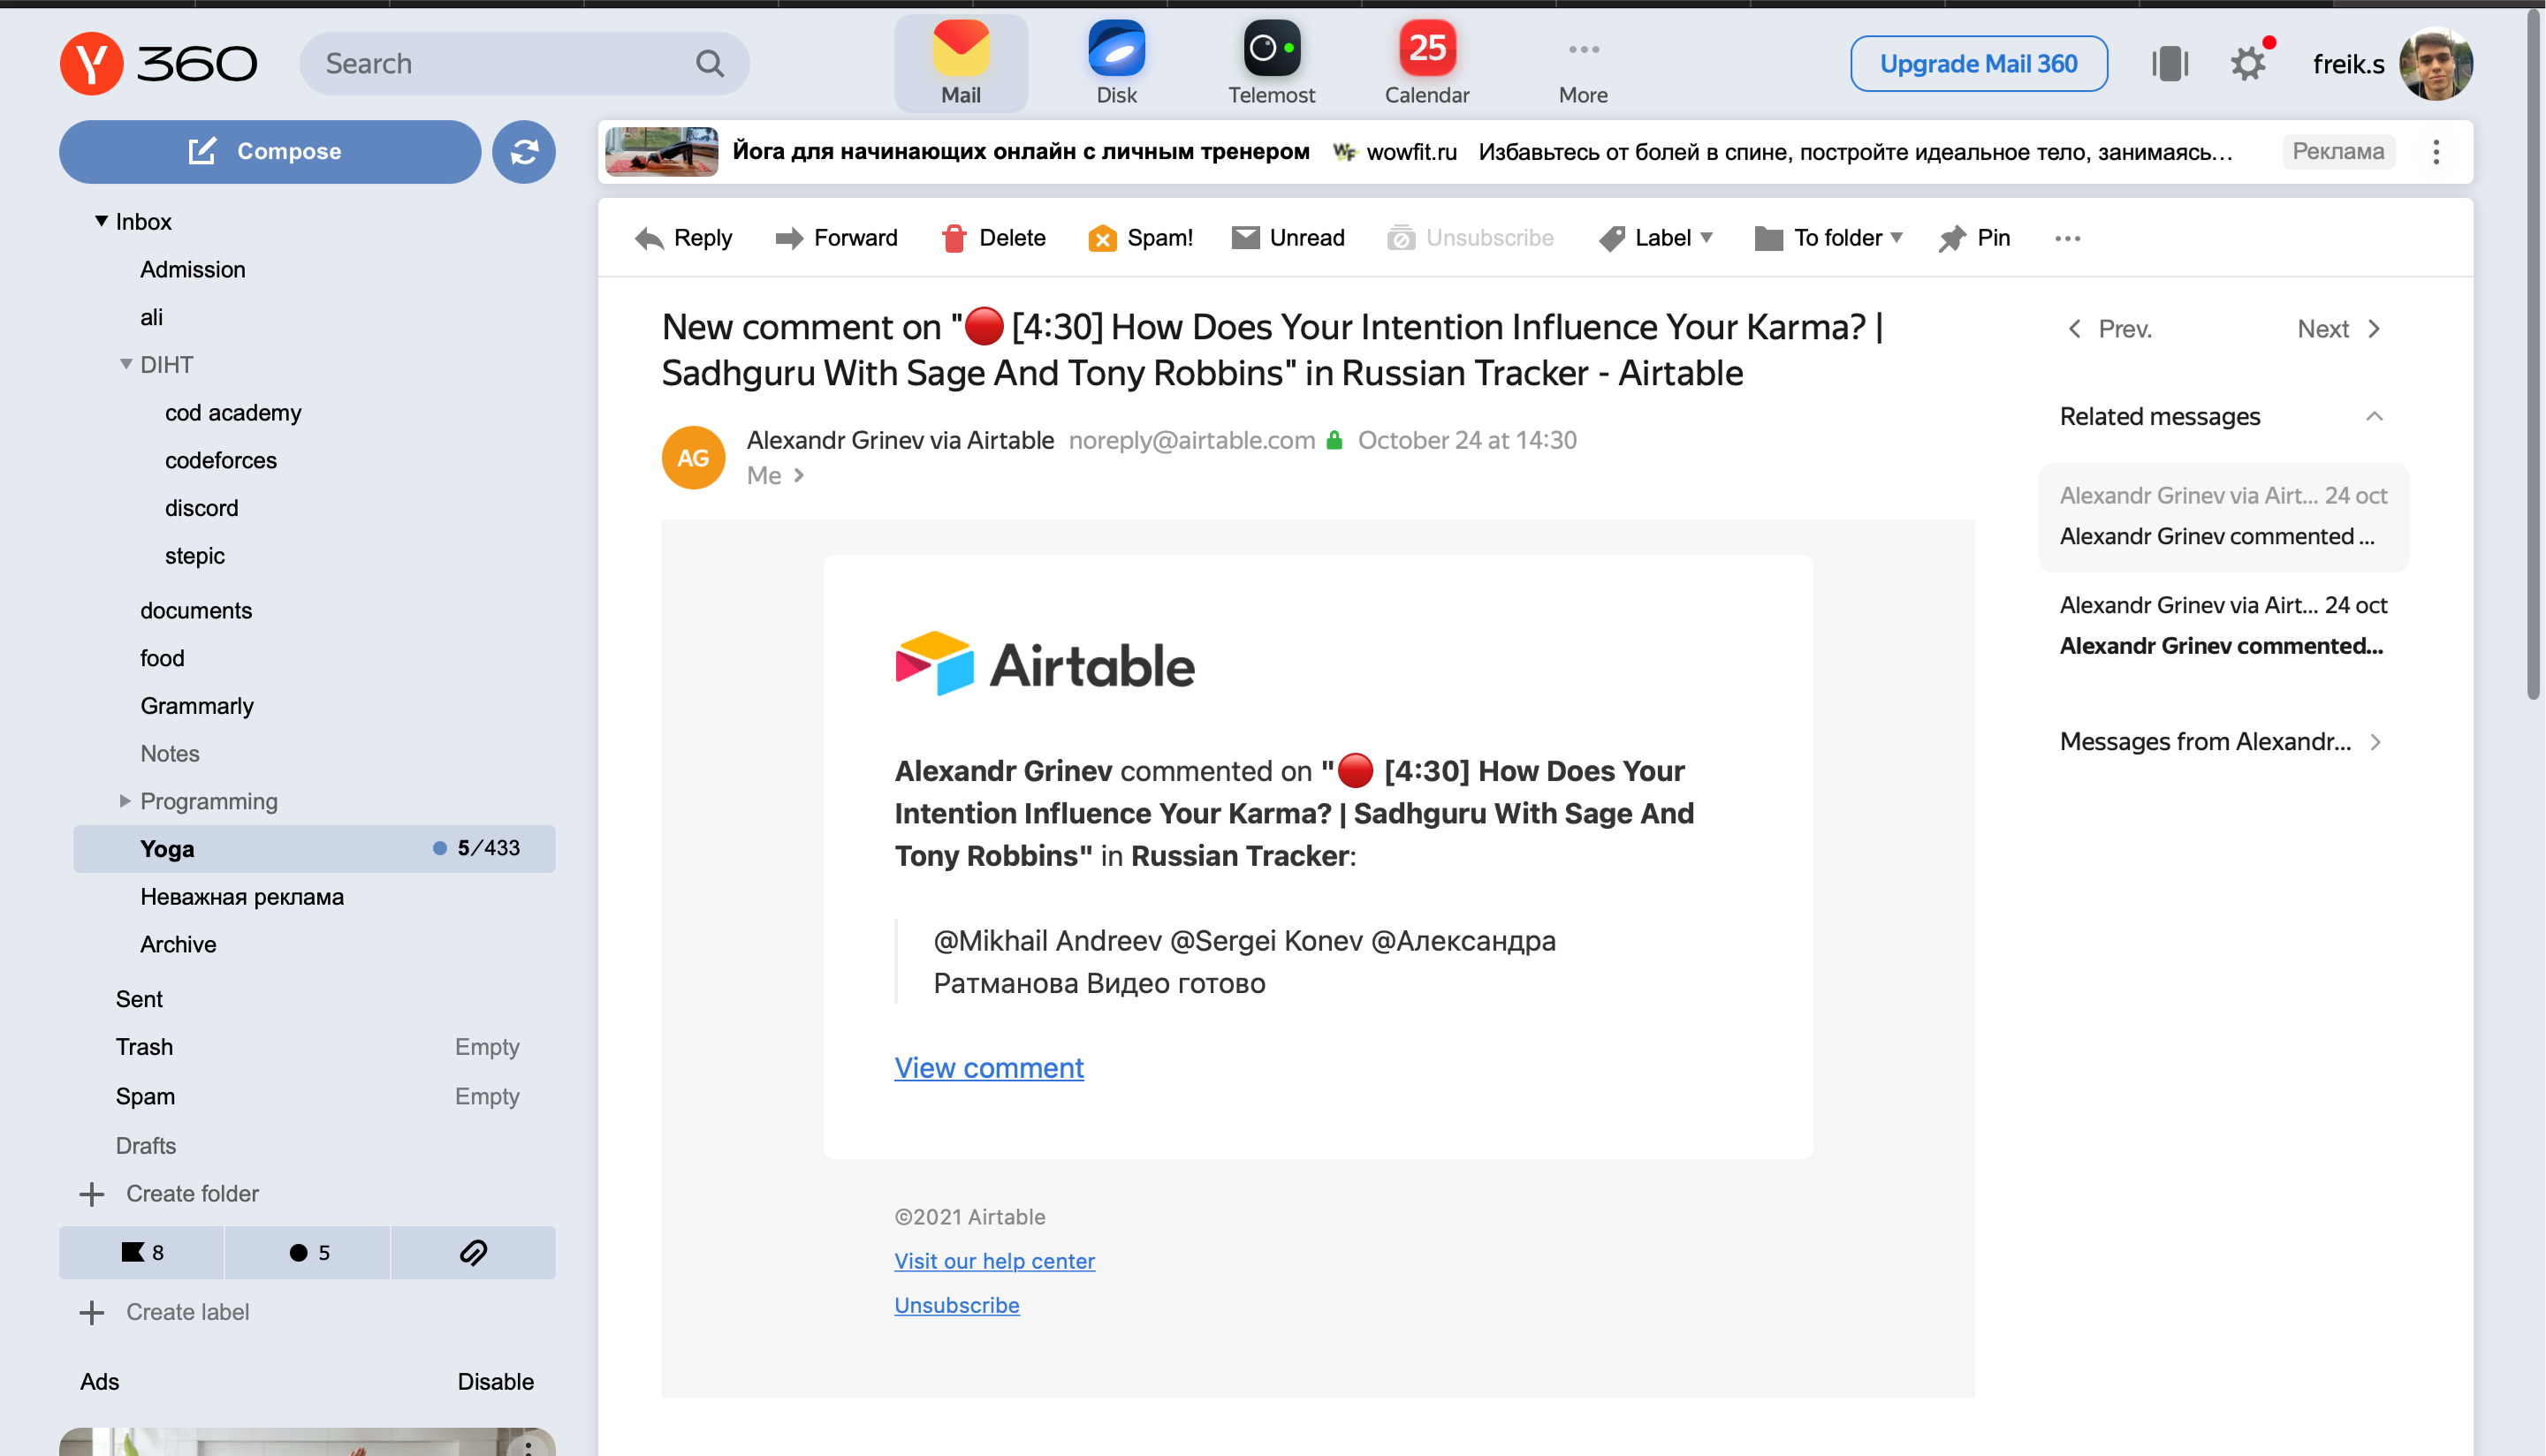
\includegraphics[width=0.9\textwidth]{AirTableSpam/ya0} 
	    \end{center}
    \item Нажмите значек \textbf{"More"} и выберите 
                \textbf{"Create filter"}.
	    \begin{center} 
	        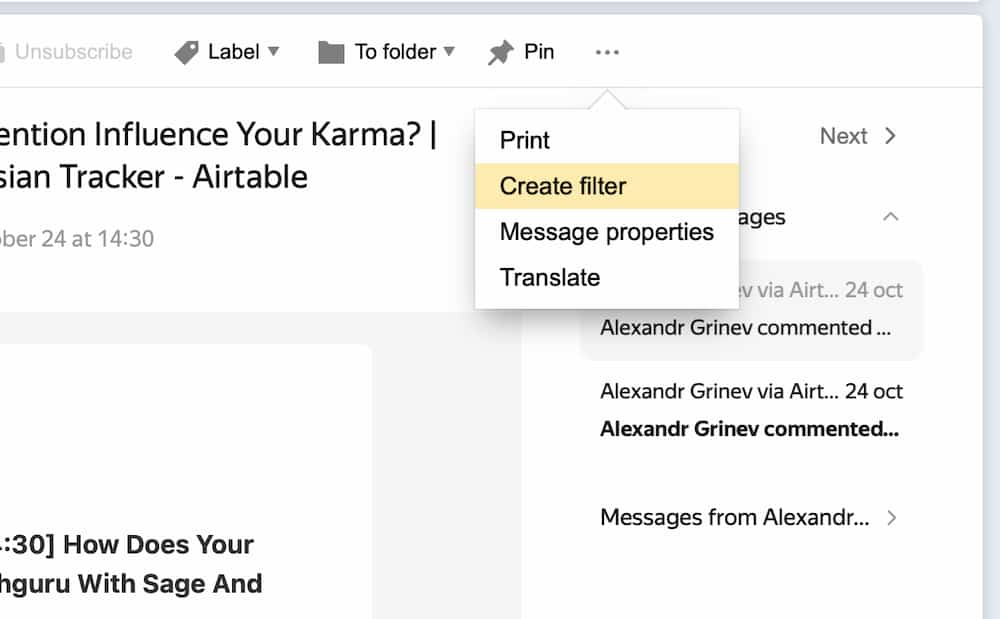
\includegraphics[width=0.5\textwidth]{AirTableSpam/ya1} 
	    \end{center}
    \item В открывшемся окне настройте параметры, как показано ниже. 
        Далее нажмите \textbf{"Create filter"}.
        \begin{itemize}
            \item Не забудьте поменять \textbf{matches} на 
                \textbf{contains} в условии 
                фильтра по предмету письма и заменить текст на 
                \textbf{"New comment on "}.
            \item Если отметить калочкой \textbf{"Apply to existing messages"},
                то фильтр применится и к нежелательным письмам, которые 
                уже пришли.
            \item Далее все письма от \textbf{"noreply@airtable.com"}, предмет
                которых которых содержит \textbf{"New comment on "} 
                будут автоматически помечаться прочитанными 
                и перемещаться в папку \textbf{"Archive"}.
        \end{itemize}

	    \begin{center} 
	        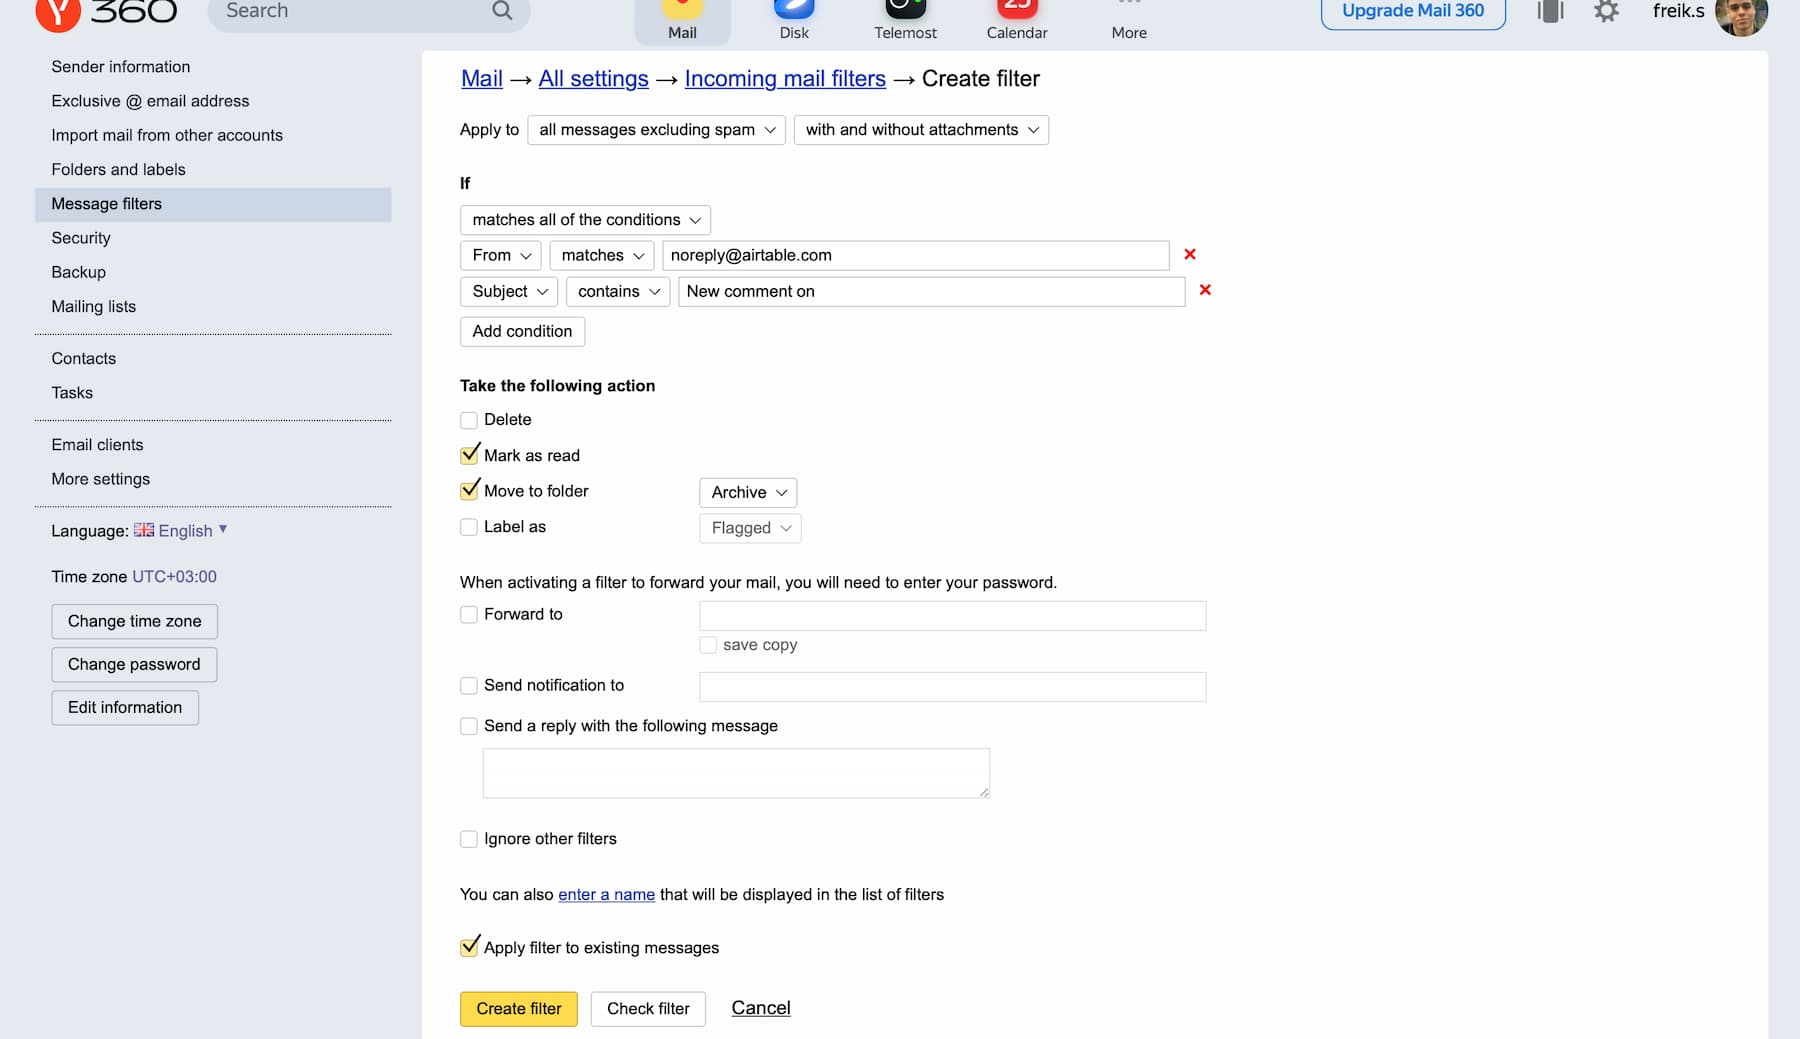
\includegraphics[width=0.9\textwidth]{AirTableSpam/ya2} 
	    \end{center}

\end{enumerate}

\thispagestyle{empty}
\tikz[remember picture,overlay] \node[opacity=0.15,inner sep=0pt] at (current page.center){
\includegraphics[width=0.2\paperwidth]{IshaLogo}};
\end{document}
%
